\section{Reinforcement Learning}
\begin{figure}[!h]
    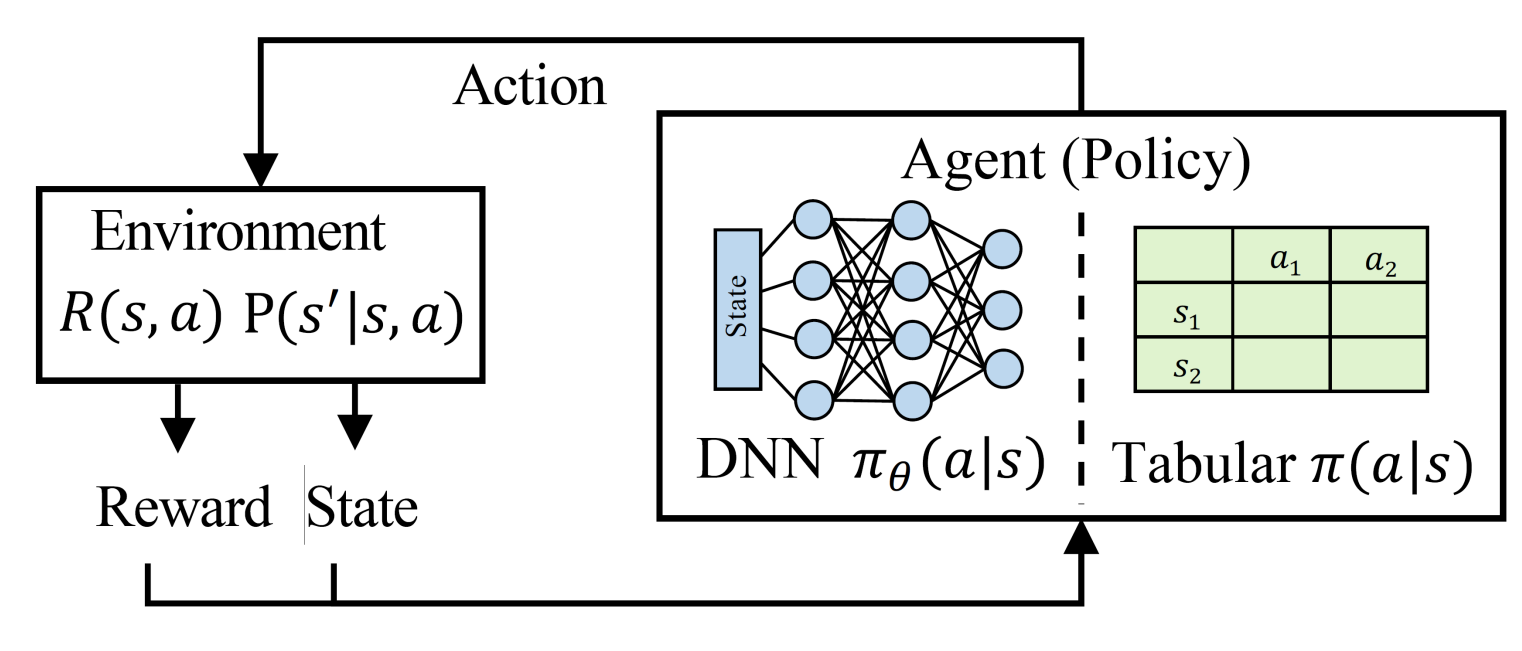
\includegraphics[width = \columnwidth]{figures/13/AgentEnvironment.png}    
\end{figure}
\begin{figure}
    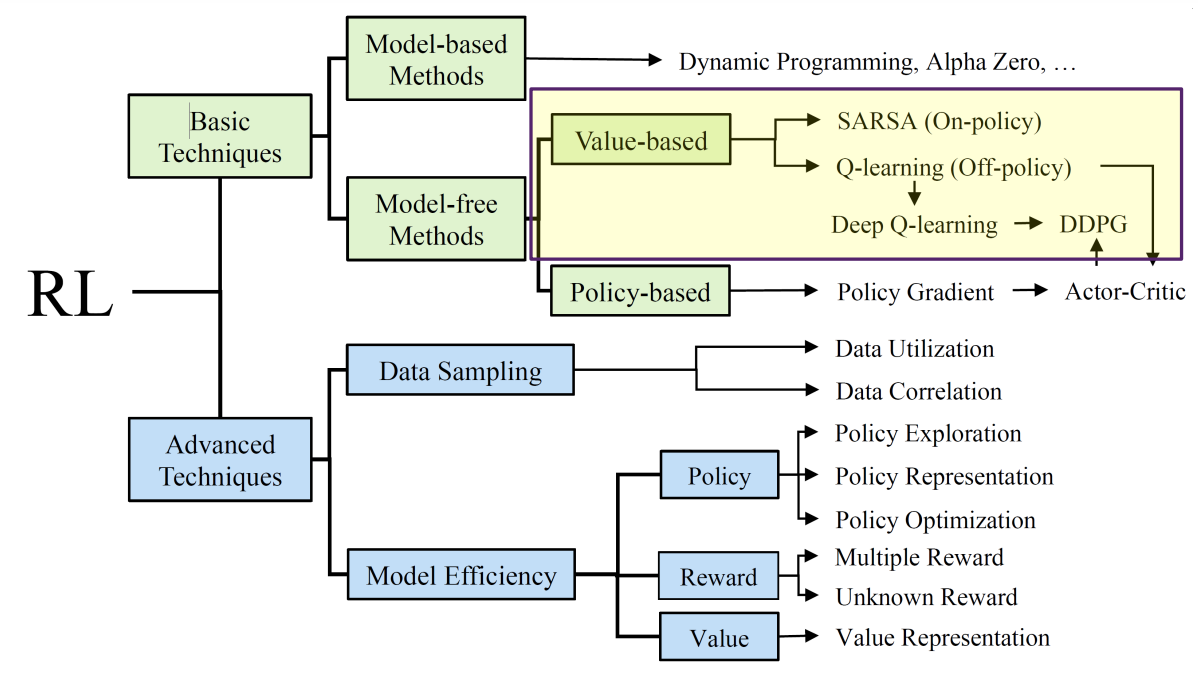
\includegraphics[width = \columnwidth]{figures/13/OverviewRL.png}
\end{figure}
The agent and environment interact at each of a sequence of discrete time steps,\(t = 0,1,2,\dots\).
At each time step \(t\), the agent receives some representation of the environment's states,\(s_i \in S\), where \(S\) is the set possible states.
On that basis, the agent selects an action, \(a\in A(s_t)\), where \(A(s_t)\) is the set of actions available in state \(s_t\).
One time step later, in part as a consequence of its action, the agent receives a numerical reward,\(R_{t+1}\in \mathbb{R}\), and finds itself in a new state, \(s_{t+1}\).
\subsubsection{Policy \(\pi\)}
A policy \(\pi\) is a distribution over actions \(a\) given state \(s\),i.e. it is the probability that the agent takes action \(a_t \in A\) in state \(s \in S\)
\[
\pi(a|s) = Pr\left[a_t = a|s_t = s\right]
\]
\subsubsection{Types of RL environments}
\begin{itemize}
    \item Deterministic environment
    \item Stochastic environment
    \item Fully observeable environment
    \item Partially observeable environment
    \item Discrete environment
    \item Continuous environment
    \item Episodic and non-episodic environment
    \item Single and multi-agent environment
\end{itemize}
\subsubsection{Agent Categories}
\begin{itemize}
    \item Value Based: No policy, Value function
    \item Policy Based: Policy, No value function
    \item Actor Critic: Policy(for the actor), Value function (for the critic)
    \item Model Free: Policy and/or Value function, no (explicit) Model of the Environment, no explicit dynamics Model
    \item Model Based: Optionally Policy and/or Value function, (explicit) Model of the Environment, explicit dynamics Model
\end{itemize}
\subsubsection{Markov Process}
A Markov Process (or Markov Chain) is a tuple (S,P), where:
\begin{itemize}
    \item \(S\) is a (finite) set of states
    \item \(P\) is a state transition probability matrix(Markov table): \(P_{ss'} = Pr(s_{t+1}|s_t)\)
\end{itemize}
The core concept is that the future only depends in the present and not on the past.
\subsubsection{Markov Reward Process (MRP)}
A Markov Reward Process is a tuple \((S,P,\mathcal{R},\gamma)\):
\begin{itemize}
    \item \(S\) is a (finite) set of states
    \item \(P\) is a state transition probability matrix:\(P = P_{ss'} = Pr(s_{t+1}|s_t)\)
    \item \(\mathcal{R}\) is a reward function (expectation value of the next reward): \(\mathcal{R}_s = \mathbb{E}\left[R_{t+1}|s_t\right]\)
    \item \(\gamma\) is a discount factor: \(\gamma \in \left[0,1\right]\)
\end{itemize}
\subsection{Markov decision process (MDP = MRP + A)}
A Markov Decision Process is a tuple \((S,A,P,\mathcal{R},\gamma)\)
\begin{itemize}
    \item \(S\) is a (finite) set of states
    \item \(A\) is a (finite) set of actions
    \item \(P\) is a state transition probability matrix:\(P = P_{ss'} = Pr(s_{t+1}|s_t)\)
    \item \(\mathcal{R}\) is a reward function (expectation value of the next reward): \(\mathcal{R}_s = \mathbb{E}\left[R_{t+1}|s_t\right]\)
    \item \(\gamma\) is a discount factor: \(\gamma \in \left[0,1\right]\)
\end{itemize}

\subsubsection{Return \(G_t\)}
The Return \(G_t\) is the total discounted reward from time-step \(t\) on.
\[
G_t = R_{t+1} + \gamma R_{t+2} + \dots = \sum_{k = 0}^{\infty} \gamma^k R_{t+k+1}
\]
\begin{itemize}
    \item \(\gamma\) close to 0 leads to myopic evaluation
    \item \(\gamma\) close to 1 leads to far-sighted evaluation
\end{itemize}
Recursion formula (basis for the Bellman equation):
\[
G_t = R_{t+1} + \gamma G_{t+1}
\]
\subsubsection{Value Function \(V(s)\) and Bellman Equation for MRP}
The state-value-function \(V(s)\) of an MRP is the expected cumulated return starting from state \(s\);
\[
V(s) = \mathbb{E}\left[G_t|s_t = s\right]
\]
The state-value-function can be decomposed in two parts.
This leads to the Bellman Equation for MRPs
\[
V(s) = \mathcal{R}_s + \gamma \sum_{s'\in S}P_{ss'}V(s') 
\]
Bellman's principle of optimality: in many mathematical optimitzation problems, the optimum (global) solution is a sequence of optimum partial solutions.

\subsubsection{State-action-value funtion \(Q(s,a)\)}
The state-action-value function \(Q(s,a)\) is a expected return starting from state \(s\), taking action \(a\), and then following policy \(\pi\).
It can be decomposed:
\begin{align*}
    Q^\pi(s,a) &= \mathbb{E}_\pi\left[G_t|s,a\right]\\
    &= \mathbb{E}_\pi\left[R_{t+1} + \gamma Q^\pi(s_{t+1},a_{t+1})|s,a\right]
\end{align*}

The Bellmen Equation for \(Q^\pi(s,a)\):
\[
Q^\pi(a,s) = \mathcal{R}_s^a + \gamma \sum_{s'\in S}P^a_{ss'}\sum_{a' \in A}\pi(a'|s')\cdot Q^\pi(s',a')
\]
\subsubsection{Maximum value function: max.expected future reward}
Goal of the MDP: the optimum policy
\[
V^*(s) = \max_{\pi}\left\{V^\pi(s)\right\}
\]
\[
Q^*(s,a) = \max_{\pi}\left\{Q^\pi(s,a)\right\}
\]
\subsection{Temporal-Difference (TD) Learning}
There are two concepts for solving Markov decision processes (MDPs).
\begin{itemize}
    \item Monte Carlo(MC) techiques
    \item Dynamic Programming(DP)
\end{itemize}
Temporal-difference (TD) learning is a combination of these two approaches. 
It learns directly from experience by sampling, but also bootstraps.
This represents a breakthrough in capability that allows agents to learn optimal strategies in any environment.
\subsubsection{Updating the Value Function}
\textbf{Monte Carlo:} The value function \(V(s)\) is updated by averaging the returns observed from multiple episodes that pass through state \(s\), where \(G_t\) is the return (cumulative discounted reward) following state \(s\) at time \(t\) and \(\alpha\) is the learning rate.
\[
V^{(t+1)}(s) = V^{(t)}(s) + \alpha\left[G_t - V^{(t)}(s)\right]
\]

\textbf{Bootstrapping methods}, such as those used in Temporal-Difference (TD) learning, update the value function based on estimates rather than waiting for the final outcome.
These methods can update the value function after each time step, leading to faster learning.

Bootstrapping TD-Learning:
\[
V^{(t+1)}(s) = V^{(t)}(s) + \alpha\left[r + \gamma V^{(t)}(s') - V^{(t)}(s)\right]
\]

Temporal-difference state-value function:
\[
V_\pi(s) = \mathbb{E}\left[V_\pi(s) + \alpha(r + \gamma V_\pi(s')-V_pi(s))|s\right]
\]

Online TD state-value estimate:
\[
V_\pi(s) \leftarrow V_\pi(s) + \alpha\left[r + \gamma V_\pi(s')\right] = V_\pi(s) + \alpha \left[V_{target} - V_\pi(s)\right]
\]

